\chapter{Results}

Our proclaimed goal for the visualization was to enable large hierarchical networks in VR. 
Therefore, we decided to test our application in a performance evaluation in Section \ref{sec:performanceEvaluation} and gather user feedback in the form of a heuristic evaluation in Section \ref{sec:heuristicEvaluation}.

\section{Performance}
\label{sec:performanceEvaluation}

Real time 3D applications need to have a constant frame rate in order to achieve a smooth experience.
For VR-based applications this is even more important as a low frame rate could lead to motion sickness. 
In our performance test, we distinguish between the duration of the initial phase when the application is started until the force based layout algorithm is finished, and the render performance during the exploration phase. 

In the performance evaluation we want to find out the scalability of our application. 
For an optimal VR experience the frame rate should be constant and equal to the maximum supported refresh rate of the VR headset's displays. In the case of the HTC Vive this requires us to have a constant frame rate of 90 FPS.
Own experiments showed that 20-30 FPS is the minimum while exploring a virtual scene without being distracted.
\\
We measured the FPS directly from the visualization by adding an FPS counter on the virtual controller model during the exploration. Our setup was a desktop PC with a Ryzen 7 3700X CPU and a Radeon RX 590 GPU. 
We tested multiple datasets with different sizes, the results are shown in Table \ref{table:resultFPS}. 
In order to detect possible performance problems, we tested the scaling of the nodes and links individually.
We found that the number of nodes scale worse than the number of links (see Figure \ref{fig:performanceNodes} and \ref{fig:performanceLinks}). 
For an equal distributed graph, the number of hierarchical layers only indirectly influence the frame rate, as with an increased number of layers the number of nodes grows exponentially.
We always apply a constant number of simulation steps, therefore at about 6 hierarchical layers the layout algorithm becomes unstable and can not guarantee a correct hierarchical nesting anymore.
\\
While the average frame rate is not drastically reduced by the amount of links, the frame rate seems to get more unstable with an increasing amount of links. 
This was especially noticeable during the teleportation animation were the frame rate dropped on a large dataset up to 20 FPS. 
We assume the automated scaling reduced the frame rate quite significantly. During the animation, the scale of nearly all objects in the scenes is updated on every frame.
Our data only shows a maximum of 90 FPS due to the headset's maximum refresh rate of 90 Hz.
\\
In conclusion, with the current state of the implementation, the visualization can support datasets up to 1500 nodes and 3000 links depending on the hardware available.
In addition, we noticed that during the exploration, the CPU and GPU utilization was not at maximum. An explanation for this could be that the application is CPU bound and further limited by a single threaded JavaScript implementation.

\begin{table}[!hbt]
    \resizebox{\textwidth}{!}{%
    \centering
    \begin{tabular}{ | c | c | c | c | c | c | c | }
        \hline
        \textbf{nodes} & \textbf{links} &\textbf{layers} &\textbf{layout duration (s)} &\textbf{min FPS} &\textbf{avg FPS}\\
        \hline
        310  & 0    & 3 & 5    & 90 & 90\\ \hline
        730  & 0    & 3 & 7,5  & 70 & 75\\ \hline
        1100 & 0    & 3 & 9,5  & 55 & 60\\ \hline
        1560 & 0    & 4 & 10,5 & 40 & 55\\ \hline
        2343 & 0    & 5 & 15   & 30 & 35\\ \hline
        774  & 387  & 3 & 10   & 60 & 70\\ \hline
        774  & 1548 & 3 & 15   & 55 & 70\\ \hline
        774  & 3870 & 3 & 27   & 40 & 60\\ \hline
        1560 & 3120 & 4 & 30   & 25 & 45\\ \hline
        1020 & 2040 & 4 & 20   & 40 & 60\\ \hline
     \end{tabular}}
     \caption[Results from the performance evaluation.]{Results from the performance evaluation, separated into duration of the layout phase in seconds and render performance in FPS during the exploration phase. Test setup: Ryzen 7 3700X + Radeon RX 590.}
     \label{table:resultFPS}
\end{table}

\begin{figure}[!hbt]
    \centering
    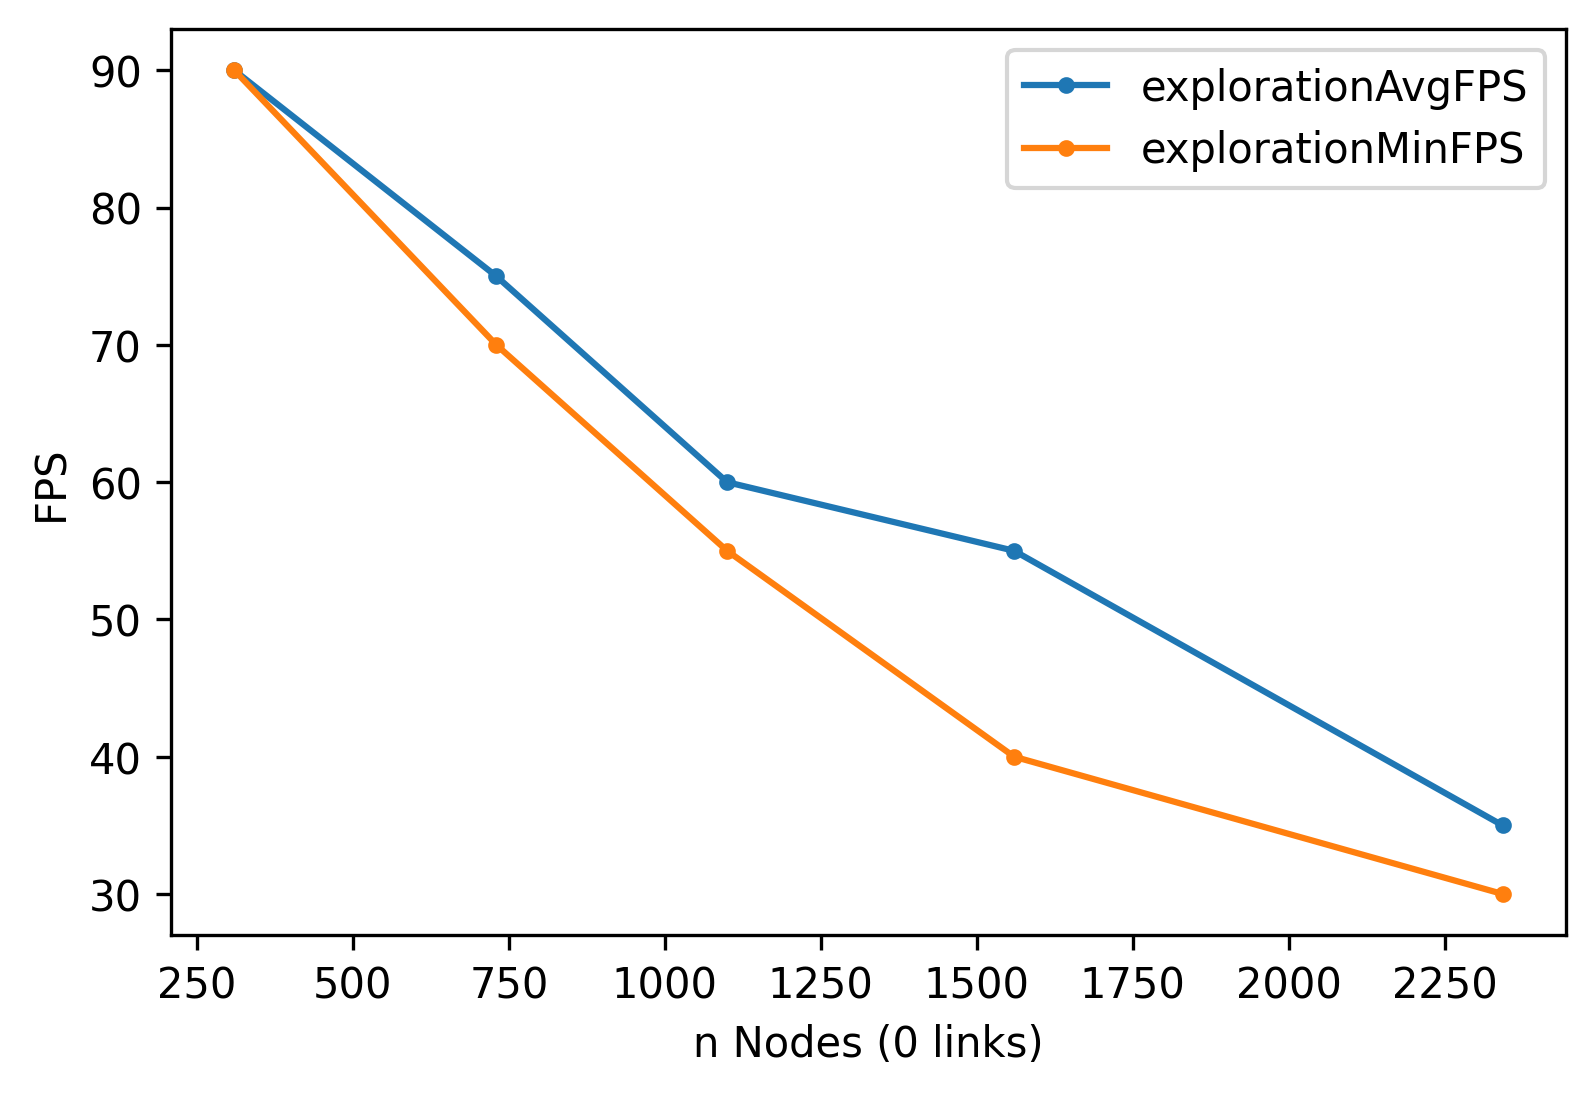
\includegraphics[width=0.75\textwidth]{graphics/performanceAnalysisNodes2.png}
    \caption[Performance chart for scaling the number of nodes.]{Performance chart for scaling the number of nodes. To better compare the results only datasets with 0 links are shown in this graph. Increasing the number of nodes quickly leads to a performance issue.} 
    \label{fig:performanceNodes} 
\end{figure}

\begin{figure}[!hbt]
    \centering
    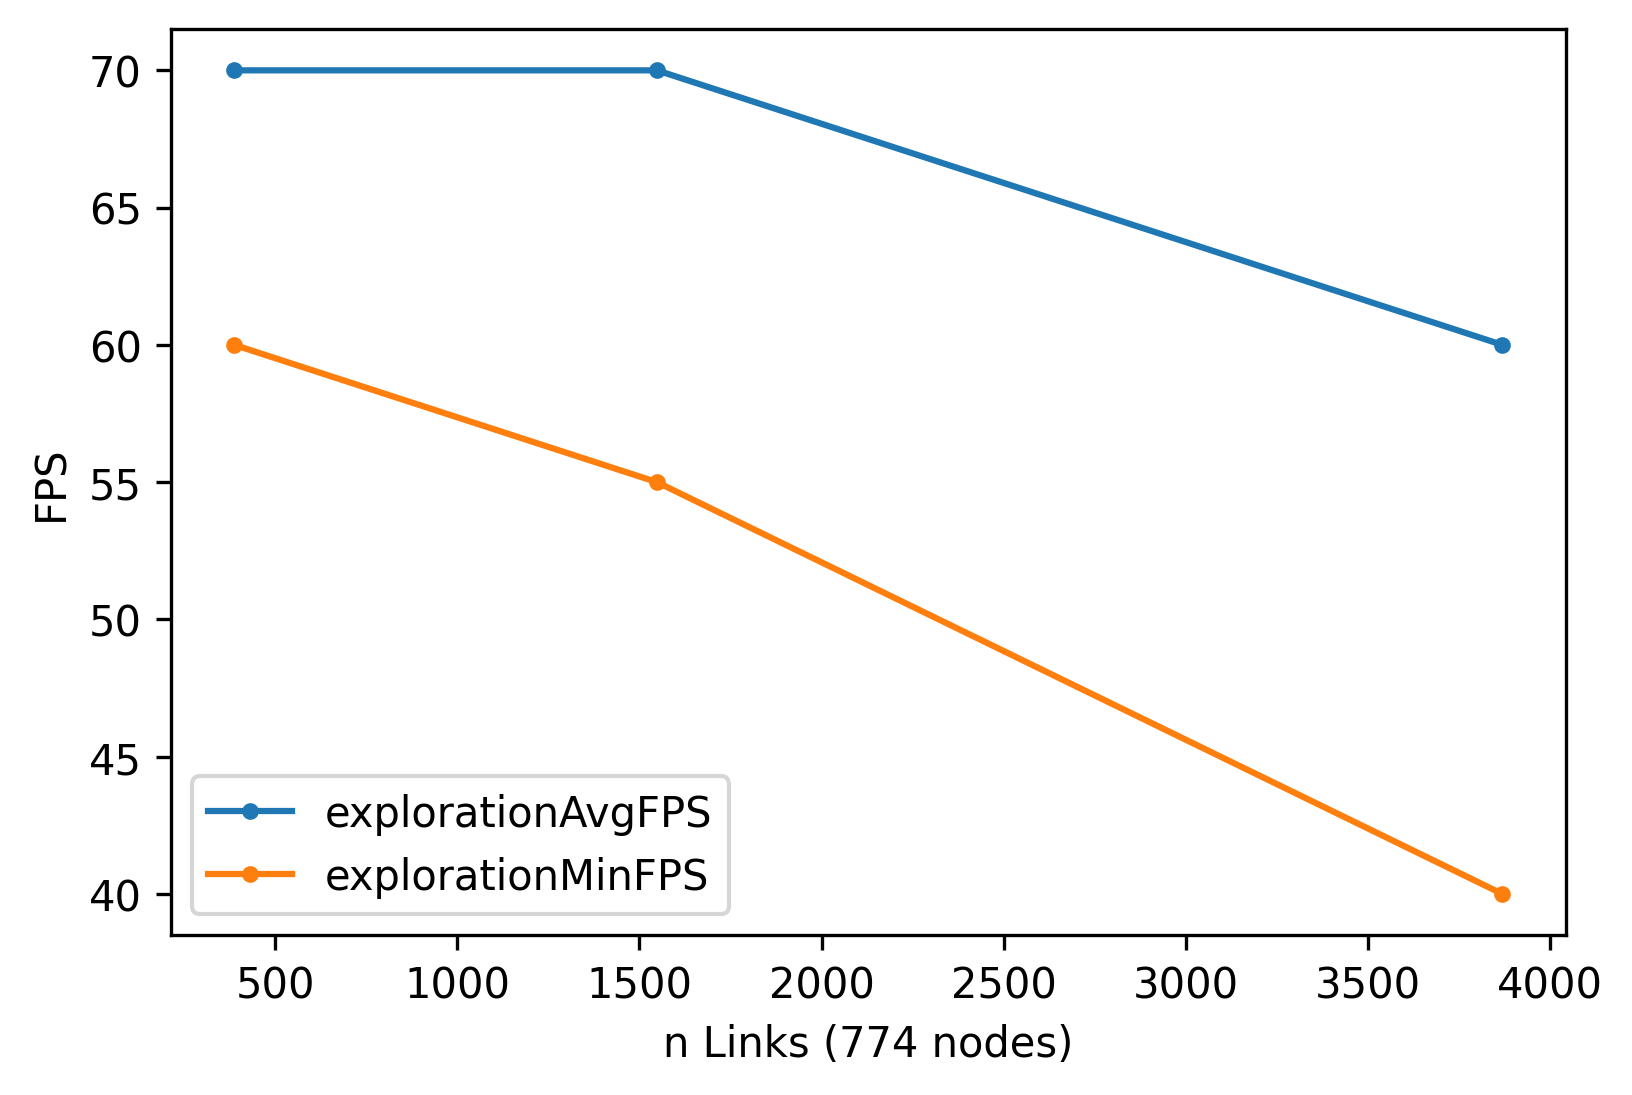
\includegraphics[width=0.75\textwidth]{graphics/performanceAnalysisLinks2.png}
    \caption[Performance chart for scaling the number of links.]{Performance chart for scaling the number of links. To better compare the results only datasets with the same amount of 774 nodes are shown in this graph. In comparison to the nodes, links can be easier scaled up without impacting the performance too much.} 
    \label{fig:performanceLinks} 
\end{figure}

\subsection{Possible optimization}

To increase the overall performance, the scalability for the number of nodes needs to be improved. We can separate the performance problems between GPU and CPU bottlenecks.
\\
To increase the GPU performance, we already limit the draw calls by rendering the nodes with instanced buffers.
However, the number of rendered triangles is still very high. 
One improvement could be to use simpler sphere models with a lower polygon count. Implementing a technique that prevents the rendering of the small nodes which can not be seen anyway could further increase GPU performance.
\\
To increase CPU performance, we have to reduce the number of tasks during each iteration of the main render loop (see Figure \ref{fig:impl_programFlow}).
A big performance issues might be the calculation of the intersected objects from ray casting by the virtual laser pointer. This could be improved by taking advantage of the hierarchical layout.
Ray intersections of child nodes from different parents are not possible. Therefore, these nodes could be excluded from the ray intersection checks. 
Another improvement could be achieved by limiting the active time of the ray casting by binding the virtual laser pointer to a button that the user actively needs to hold while selecting objects. 
That would enable an improved frame rate when the user is only looking around without using the virtual laser pointer.
\\
Besides performance improvements to the techniques themselves, improving the internal data structure would also increase the performance. Based on the prior implementation, we use a flat list similar to the JSON seen in Section \ref{lst:internalJSON}. With a tree data structure that directly represents the hierarchical relationships, our internal algorithms can be implemented more efficiently when accessing the node details, therefore reducing the workload on the main render loop and increasing the FPS.

\section{Heuristic Evaluation}
\label{sec:heuristicEvaluation}

The focus of this thesis was to develop a new visualization technique, this included a hierarchical layout and VR optimized navigation and interaction techniques.
The application should deliver a smooth and user-friendly visualization.
As the application runs in the browser, we set up a website \cite{thesisWebsite} with an introduction to the topic, instructions on how to start and interact with the visualization and the option to try out the application with multiple datasets of various sizes. Afterwards we invited users to participate in the evaluation and fill out an online form that we prepared beforehand.
\\
Besides online evaluation, we also had one participant that tried the visualization on site. During and after the exploration we conducted an interview.
The results of the interview as well as the online forms are presented in the following subsections.
\\
   
\subsection{Clarity of the visualization}
Filtering, visual clutter, hierarchical layout(intuitive?), ...

\subsection{Navigation}
Free fly, animated teleport, scaling, motion sickness.

\subsection{Interaction}
Button Mappings, Laser Pointer, 

\subsection{Performance}
Tested system and dataset